\documentclass[../../main.tex]{subfiles}
\begin{document}

\subsection*{8.11}
Un conduttore cilindrico cavo di raggi a e b è percorso da una corrente distribuita uniformemente.\\
Calcolare il campo magnetico B(r) in funzione della distanza $r$ dall'asse.\\
Ricavare i risultati relativi ad un conduttore cilindrico pieno.\\
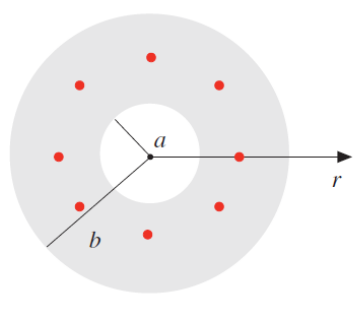
\includegraphics[scale=0.3]{e_8_11_0.png}\\
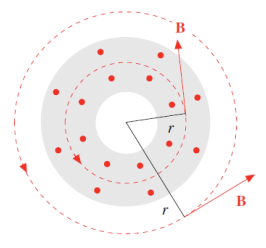
\includegraphics[scale=0.3]{e_8_11_1.png}
\subsubsection*{Formule utilizzate}
\subsubsection*{Soluzione punto a}
\subsubsection*{Soluzione punto b}
\newpage

\end{document}